\section{Lecture 1}


\subsection{Knots and knots invariants}

\paragraph{Historical remarks.} At a certain point, people thought the periodic table of chemistry elements is related to different types of knots. Peter Tait tried to build a complete table of knots (under the equivalence relation that two knots are the same if you can smoothly deform one to another). It turned out that this endeavor is not related to the periodic table but is useful in a different context.


\begin{definition}
  A \textbf{knot} is an embedding of a circle $S^1$ into $\mathbb{R}^3$ (equivalently, $S^3$) with no self-intersections. A \textbf{link} is an embedding of several circles into $\mathbb{R}^3$ with no intersections.   
\end{definition}

\begin{definition}
  Two knots are \textbf{topologically equivalent} if there is a \textbf{regular isotopy} between them.
\end{definition}


\begin{remark}
    Note that in using regular isotopies (instead of isotopies) we should think of knots as being thickened to ribbons.
\end{remark}


\begin{definition}
  A \textbf{knot invariant} is a mapping from the set of all knots to some output set $X$ such that two topologically equivalent knots give the same result in $X$. 
\end{definition}

\begin{remark}
    Two elements in $X$ would ideally be easy to compare equality, so that different outputs would imply that the two knots are not topologically equivalent. 
\end{remark}

\begin{example}[Kauffman bracket invariant]
  Let $A$ be a scalar variable and set $d = -A^2 -A^{-2}$. We have the following rules:
  \begin{itemize}
    \item A disjoint union of $n$ unknots is replaced with $d^n$;
    \item An undercrossing and an overcrossing can be replaced as follows.
  \end{itemize}
  \begin{center}
	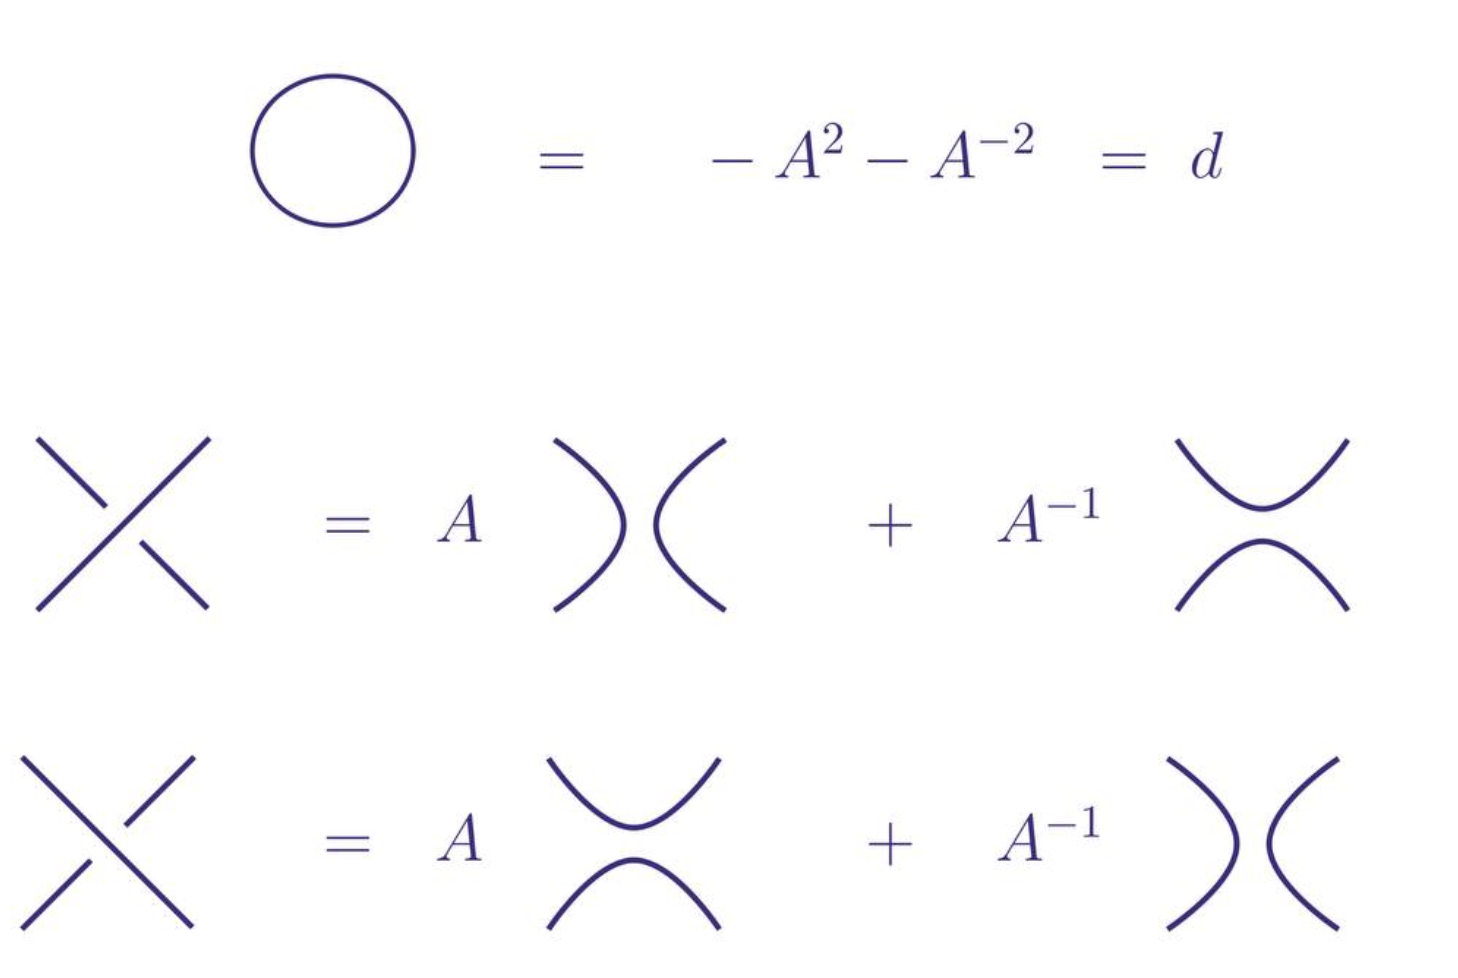
\includegraphics[width=.5\linewidth]{img/1-14-27-14.png}
\end{center}
\end{example}


\begin{proposition}
  The Kauffman bracket is a knot invariant.
\end{proposition}

There is no proof for now.


\begin{remark}
    The Kauffman bracket is not invariant under type I Reidemeister moves; but since we only consider regular isotopies here, type I moves are not included.
\end{remark}

An example calculation is on p.5 of the book.
If we calculate this naively, the time complexity is $O(2^N)$, where $N$ is the number of crossings in the knot; this is pretty bad.


\subsection{Relation to physics}

Consider two-dimensional systems plus one dimension of time, which we call $(2+1)$-dimensional systems. We can consider events in a disk. First there is a pair of creation event: a particle-antiparticle appear from the vacuum, and then another pair creation event. Then one particle walks around another, and the pairs come back together to try to reannihilate. At the end, there is some probability amplitude that the reannihilation is successful, but it is also possible that it is not. In a topological theory, this probability amplitude depends only on the topology of worldlines and not on the geometry of the paths. 

If a quantum computation system is topological, it is less vulnerable to noise disturbance.
